\section{Siamese Network}

Siamese networks, first introduced by Bromley \cite{bromley1993signature} in 1993, contains multiple instances of the same model and share the same configuration and weights. The term “siamese twins,” means “conjoined twins,” which is two identical twins connected in utero. These twins share the same organs. Each sub-network is a typical Convolutional Neural Network (CNN), as shown in figure \ref{fig:cnn}. A CNN usually contains an input layer, an output layer, and multiple hidden layers. The hidden layers consist of convolutional layers, pooling layers, fully connected layers, and normalization layers (ReLU). 

The siamese networks accept distinct inputs and learn their feature vectors, joined by an energy function at the top. This function computes the similarity between the highest-level feature representation on each side. Parameter updates are mirrored across the twin networks. This means if the weights on one network are updated, then the weights on the other one are also updated. It guarantees the two similar inputs will not be mapped by each network to different locations in feature space. Furthermore, instead of training a classification model to classify the dataset into correct categories, it asks the model to recognize if the two inputs are similar or not. It means that the siamese network architectures do not need to concern themselves with classification to select 1 of N possible classes, like the traditional classification model. Rather, they only answer whether the two inputs are similar or not. Based on the characteristics, siamese networks perform well in the scenario that the dataset consists of numerous categories but in which each class has few samples. Therefore, siamese networks have been successfully applied to address face recognition \cite{schroff2015facenet}, image retrieval, person re-identification \cite{fang2019bilinear}, localization \cite{tompson2015efficient}, and even object tracing \cite{bertinetto2016fully} tasks. 


\begin{figure}[h]
  \centering
  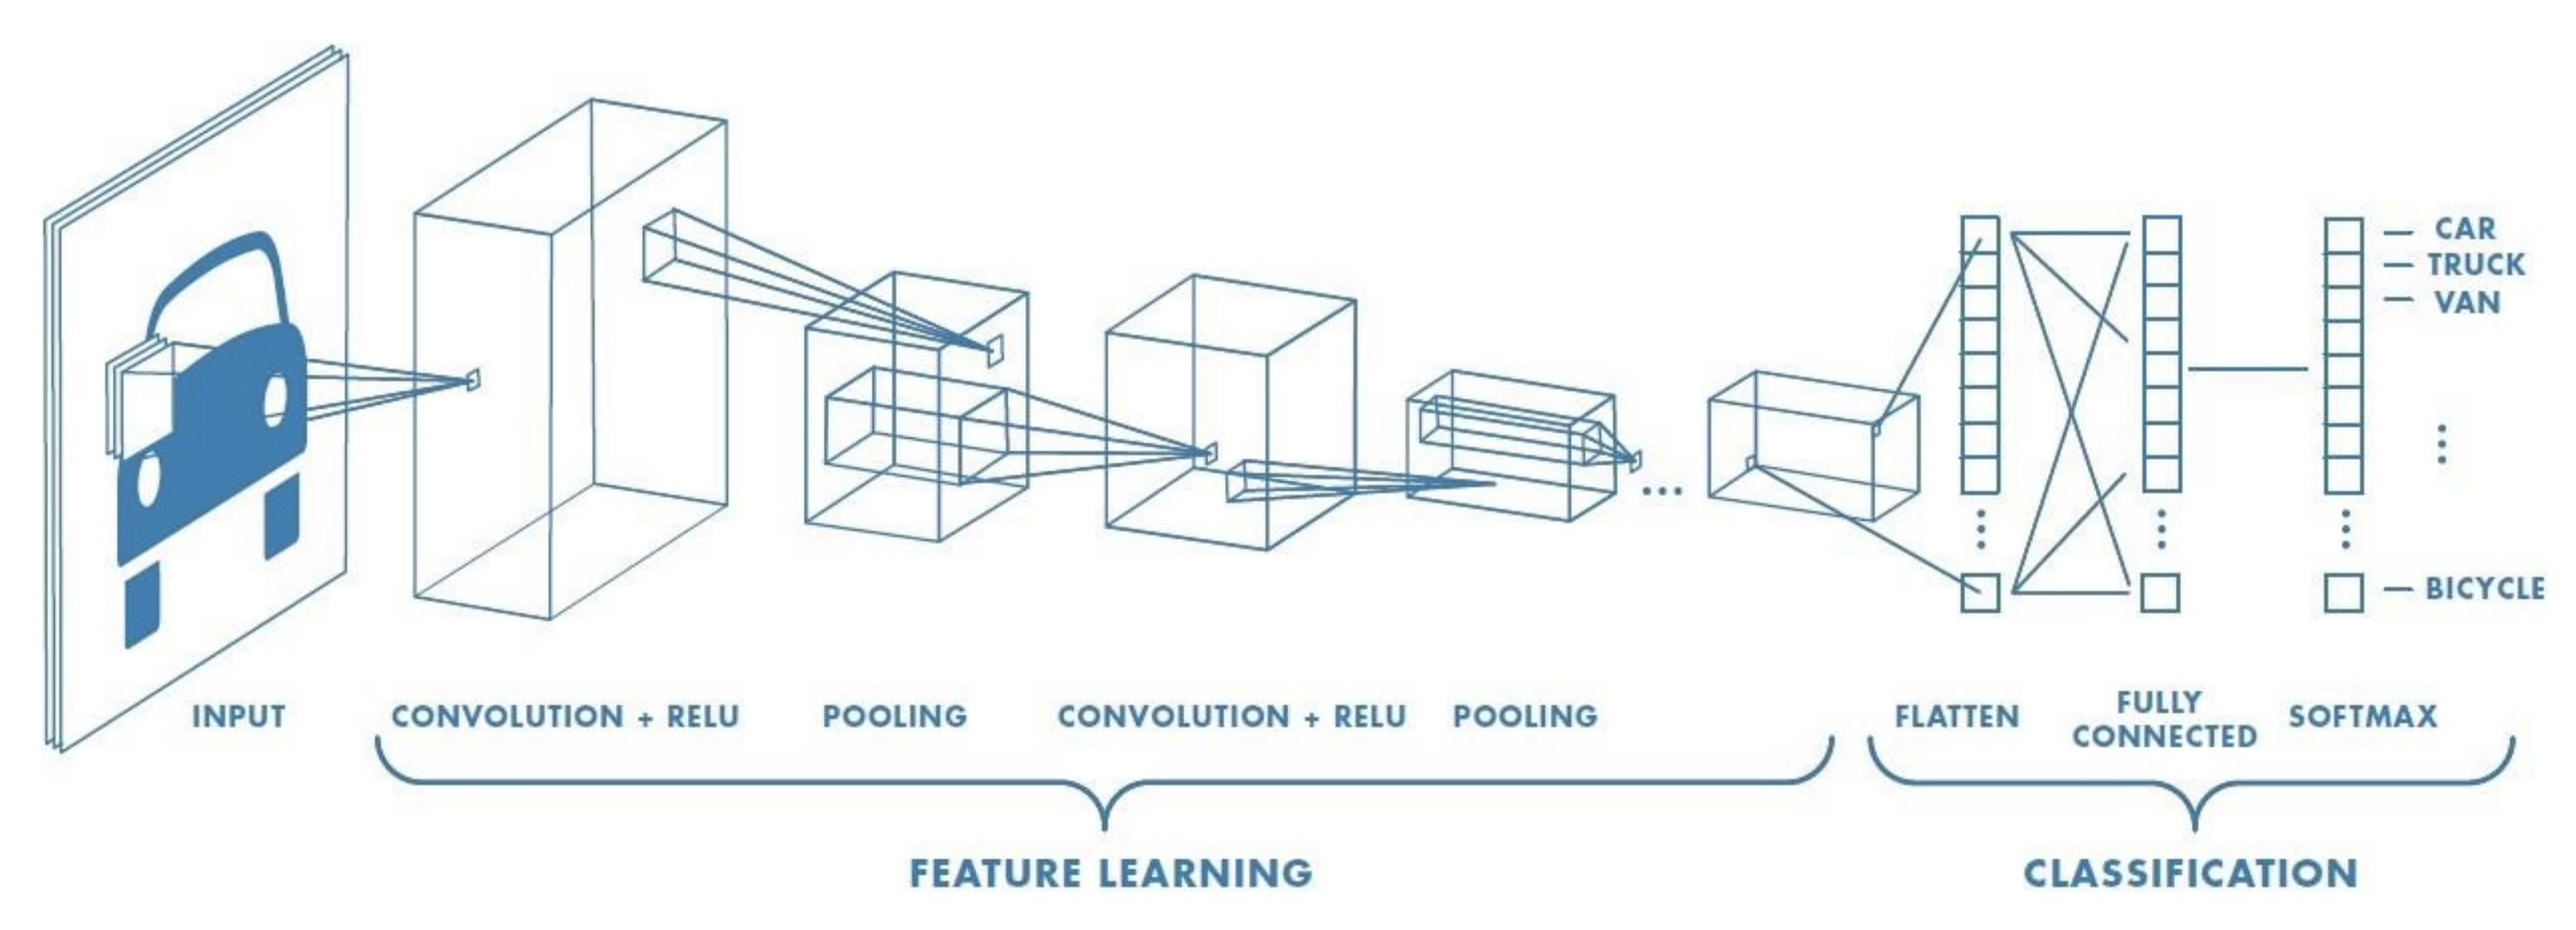
\includegraphics[width=\linewidth]{figs/cnn.png}
  \caption{A typical Convolutional Neural Network (CNN) architecture.}
  \label{fig:cnn}
\end{figure}

In most cases, the siamese networks have a strong embedding capability to learn a non-linear embedding of data to obtain semantically meaningful spaces. In these spaces, the related patterns of similar objects are close to each other while unrelated patterns of different objects are far away from each other. In general, the training of the siamese network is accomplished by two steps: 1) learning non-linear embeddings of inputs, 2) followed by distance-based loss functions. The loss functions usually aim at constraining the learned embeddings to have shorter distances among samples of the same category than the distances of the distinct categories \cite{medela2019constellation}. There are several widely used distance-based loss functions, contrastive loss function \cite{sohn2016improved}, triplet loss \cite{schroff2015facenet}, multiclass-N-pair loss function \cite{chopra2005learning} and so on. The objective of these loss functions is to predict the relative distance between inputs instead of directly a label or a value given an input. The contrastive loss function measures pairs of samples. The triplet loss function is extended to compare a sample with its positive and negative samples. Meanwhile, the multiclass-N-pair loss function is to improve distance loss functions by generalizing triplet loss. The distance-based loss function selection is very flexible in terms of the dataset. 

In this project, we applied the contrastive loss function and triplet loss function into siamese networks. Because they are the two most frequently used loss functions, as detailed below. 

\subsection{Contrastive Loss}
The training process with contrastive loss function is depicted in figure \ref{fig:contrastive}. The model takes image pairs as its inputs, which contain both the positive pairs and negative pairs. From the figure, it's clear that the positive pairs are composed of an anchor sample and a positive sample that is similar to the anchor. In contrast, the negative pairs contain an anchor sample and a negative sample which is dissimilar to the anchor. The objective of this model is to learn representations with a shorter distance between the positive pairs than the negative ones. Formally, the model transforms the image pairs $x_{1,i}, x_{2,i}$ into embedding vectors $v_{1,i}, v_{2,i}$, $i \in (1, N)$, where $N$ is the batch size. The contrastive loss tries to force positive pairs have 0 distance, and negative pairs have a distance greater than a margin $m$. Let $d$ be the distance function, the loss can be expressed by formula \ref{equ:loss}: 

\begin{equation}
L_i = \left\{
\begin{aligned}
 & d(v_{1,i}, v_{2,i}) \ i \in (1, N) \ \ \ \ \text{if positive pairs} \\
 & max(0, m - d(v_{1,i}, v_{2,i}) \   i \in (1, N) \ \  \  \text{if negative pairs} \\
\end{aligned}
\right.
\label{equ:loss}
\end{equation}

For positive pairs, zero loss means the model generates embeddings for both two samples with no distance between them. The corresponding parameters update, therefore, to increase the distance. For negative pairs, zero loss indicates that the distance between the embeddings of the two samples is larger than the margin $m$. Otherwise, the loss is a positive value and the model will update the related parameters to increase the distance for them. As shown in the figure \ref{fig:contrastive}, similar objects are pushed closer together while the dissimilar objects are push away from each other until the distance is larger than the margin $m$. From the formula, we observe that the largest loss of negative pairs is $m$ when the distance between the two samples is 0. Note that, there is no need to increase the distance between the negative pairs when it's already larger than the marge $m$. In doing so, we can save efforts to train other difficult parts. 

Assume $y_i$ is the binary label that equals 1 for a positive pair and 0 for a negative pair. And distance is the euclidian distance. The contrastive loss function is as formula \ref{equ:contrastive}.

\begin{equation}
L = \frac{1}{2N}\sum_{i=1}^{N}[y_i || v_{1,i} - v_{2,i} ||_2^2 +  (1 - y_i)\{ max(0, m - ||v_{1,i} - v_{2,i}||_2^2) \}]
\label{equ:contrastive}
\end{equation}

\begin{figure}[h]
  \centering
  \begin{subfigure}[b]{\linewidth}
  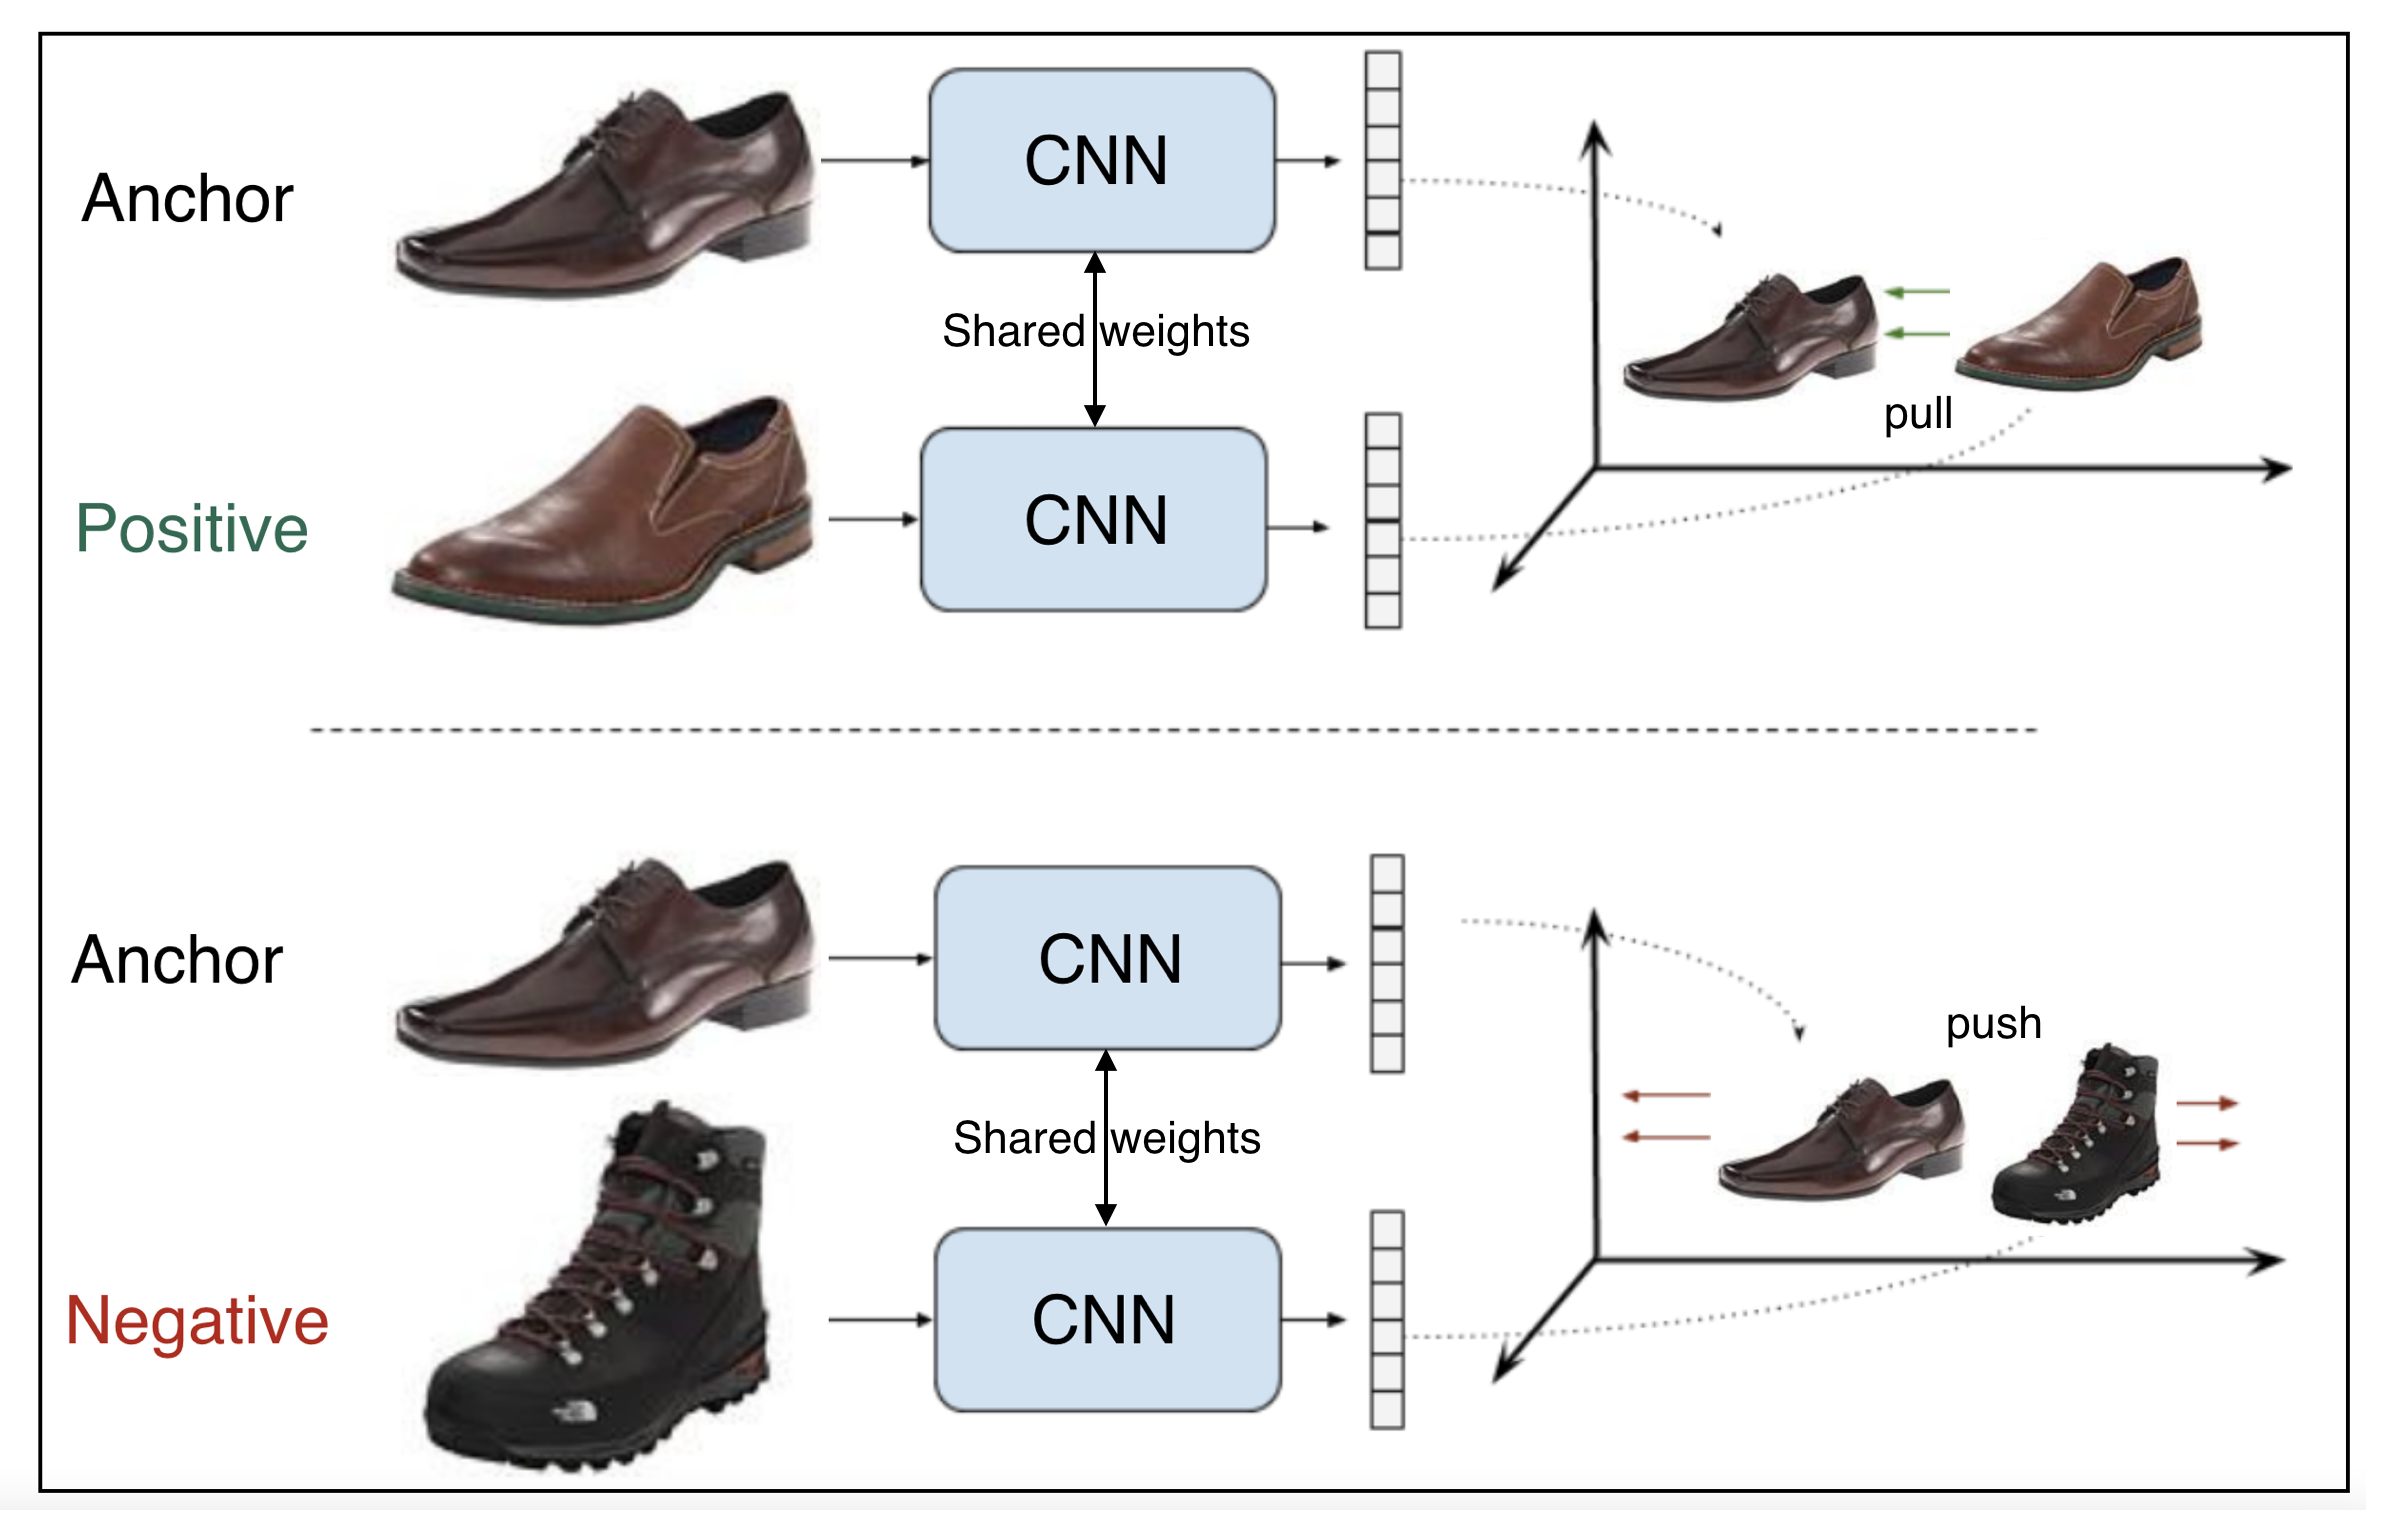
\includegraphics[width=\linewidth]{figs/contrastive.png}
  \caption{Training with contrastive loss function}
  \label{fig:contrastive}
  \end{subfigure}
  \hfill
    \begin{subfigure}[b]{\linewidth}
   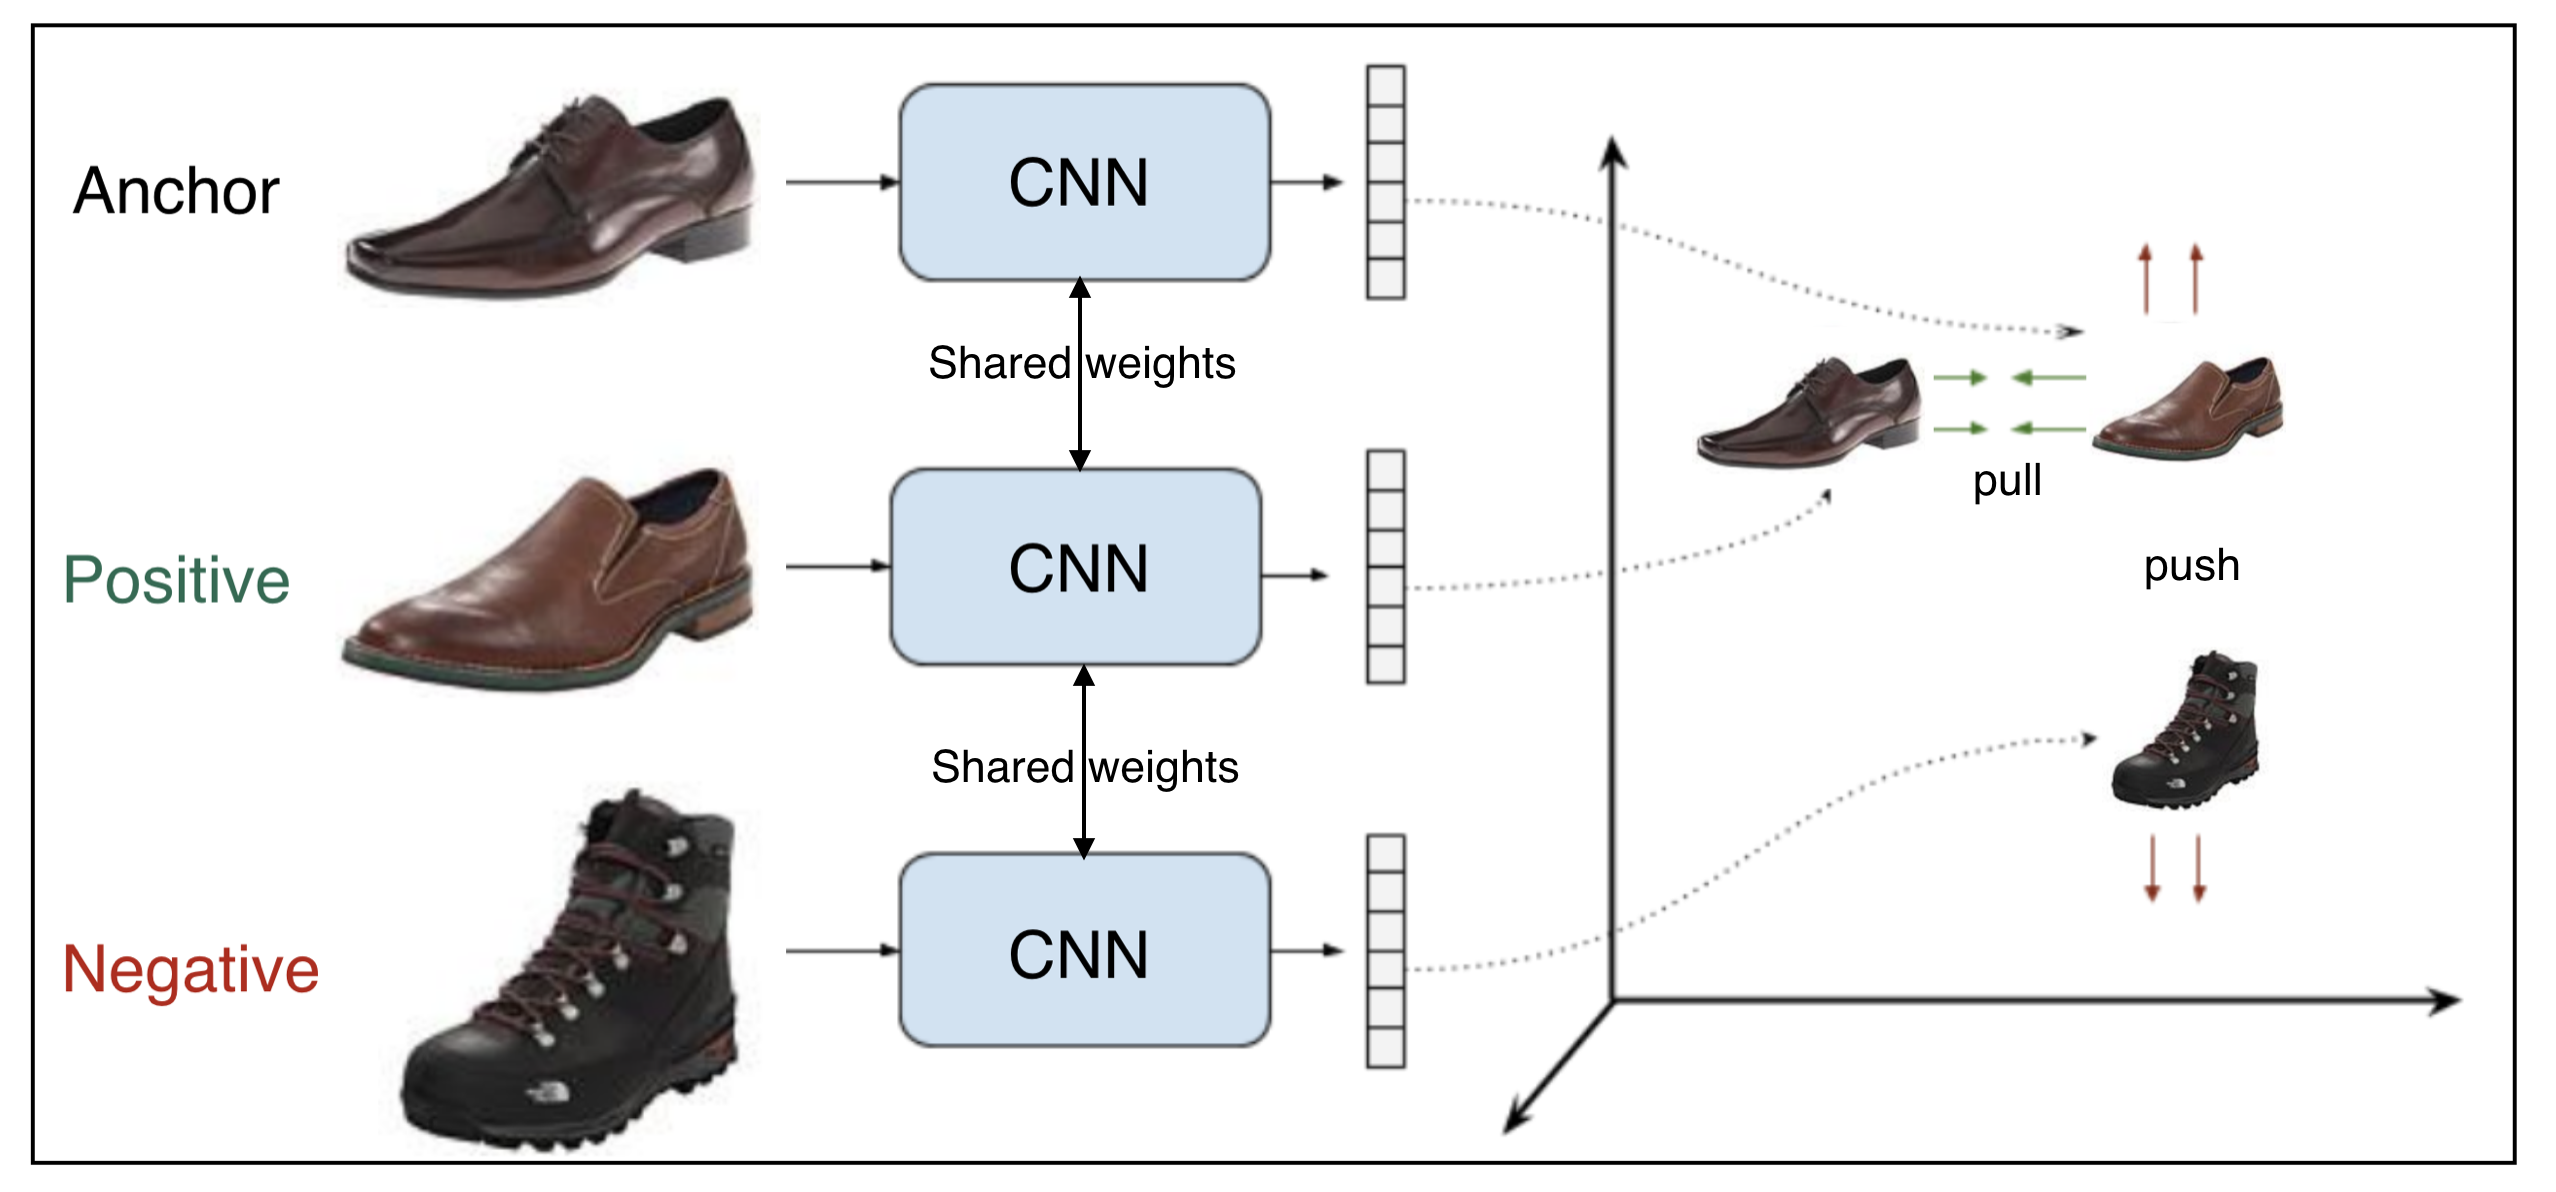
\includegraphics[width=\linewidth]{figs/triplet.png}
   \caption{Training with triplet loss function}
   \label{fig:triplet}
  \end{subfigure}
  \hfill
    \caption{Visual representation of training siamese network with different loss functions.}
    \label{fig:sialoss}
\end{figure}

\subsection{Triplet Loss}

Triplets loss function goes further by considering positive and negative pairs at the same time. The training process is shown by figure \ref{fig:triplet}. We can see that the model with triplets loss uses triplets of training samples, instead of pairs. A triplet consists of an anchor, a positive sample, and a negative sample. The goal is to minimize the distance between the anchor sample and the positive sample while maximizing the distance between the anchor sample and the negative sample. Assume $x_{a,i}, x_{p,i}, x_{n,i}$ are the anchor sample, positive sample and negative sample in a triplet respectively. $v_{a,i}, v_{p,i}, v_{n,i}$ are their correspondent embedding vectors. Note that there are no needed labels. The loss function could be as followed. 

\begin{equation}
L = \frac{1}{N}\sum_{i=1}^{N}max(0, || v_{a,i} - v_{p,i} ||_2^2 - || v_{a,i} - v_{n,i} ||_2^2  + m )
\label{equ:triplet}
\end{equation}

where $m$ is the marge and $N$ is the batch size. 

As shown in the figure \ref{fig:triplet}, at each iteration, the anchor sample is pushed closer to the positive sample while, at the same time, it is pushed away from a negative object until its distance is bigger than the margin $m$. Moreover, there are three situations of this loss, easy-triplets, hard-triplets, and semi-hard-triplets. Support the distance between the embeddings of anchor sample  $v_{a}$ and positive sample $v_{p}$ is $d(v_a, v_p)$, and the distance between negative sample $v_n$ is $d(v_a, v_n)$. The definition of easy-triplets is $d(v_a, v_n) > d(v_a, v_p) + m$, hard-triplets is $d(v_a, v_n) < d(v_a, v_p)$, and semi-hard-triplets is $d(v_a, v_p) < d(v_a, v_n) < d(v_a, v_p) + m$. Figure \ref{fig:sitiations} illustrates the relationship of these three situations. 

\begin{figure}[h]
  \centering
  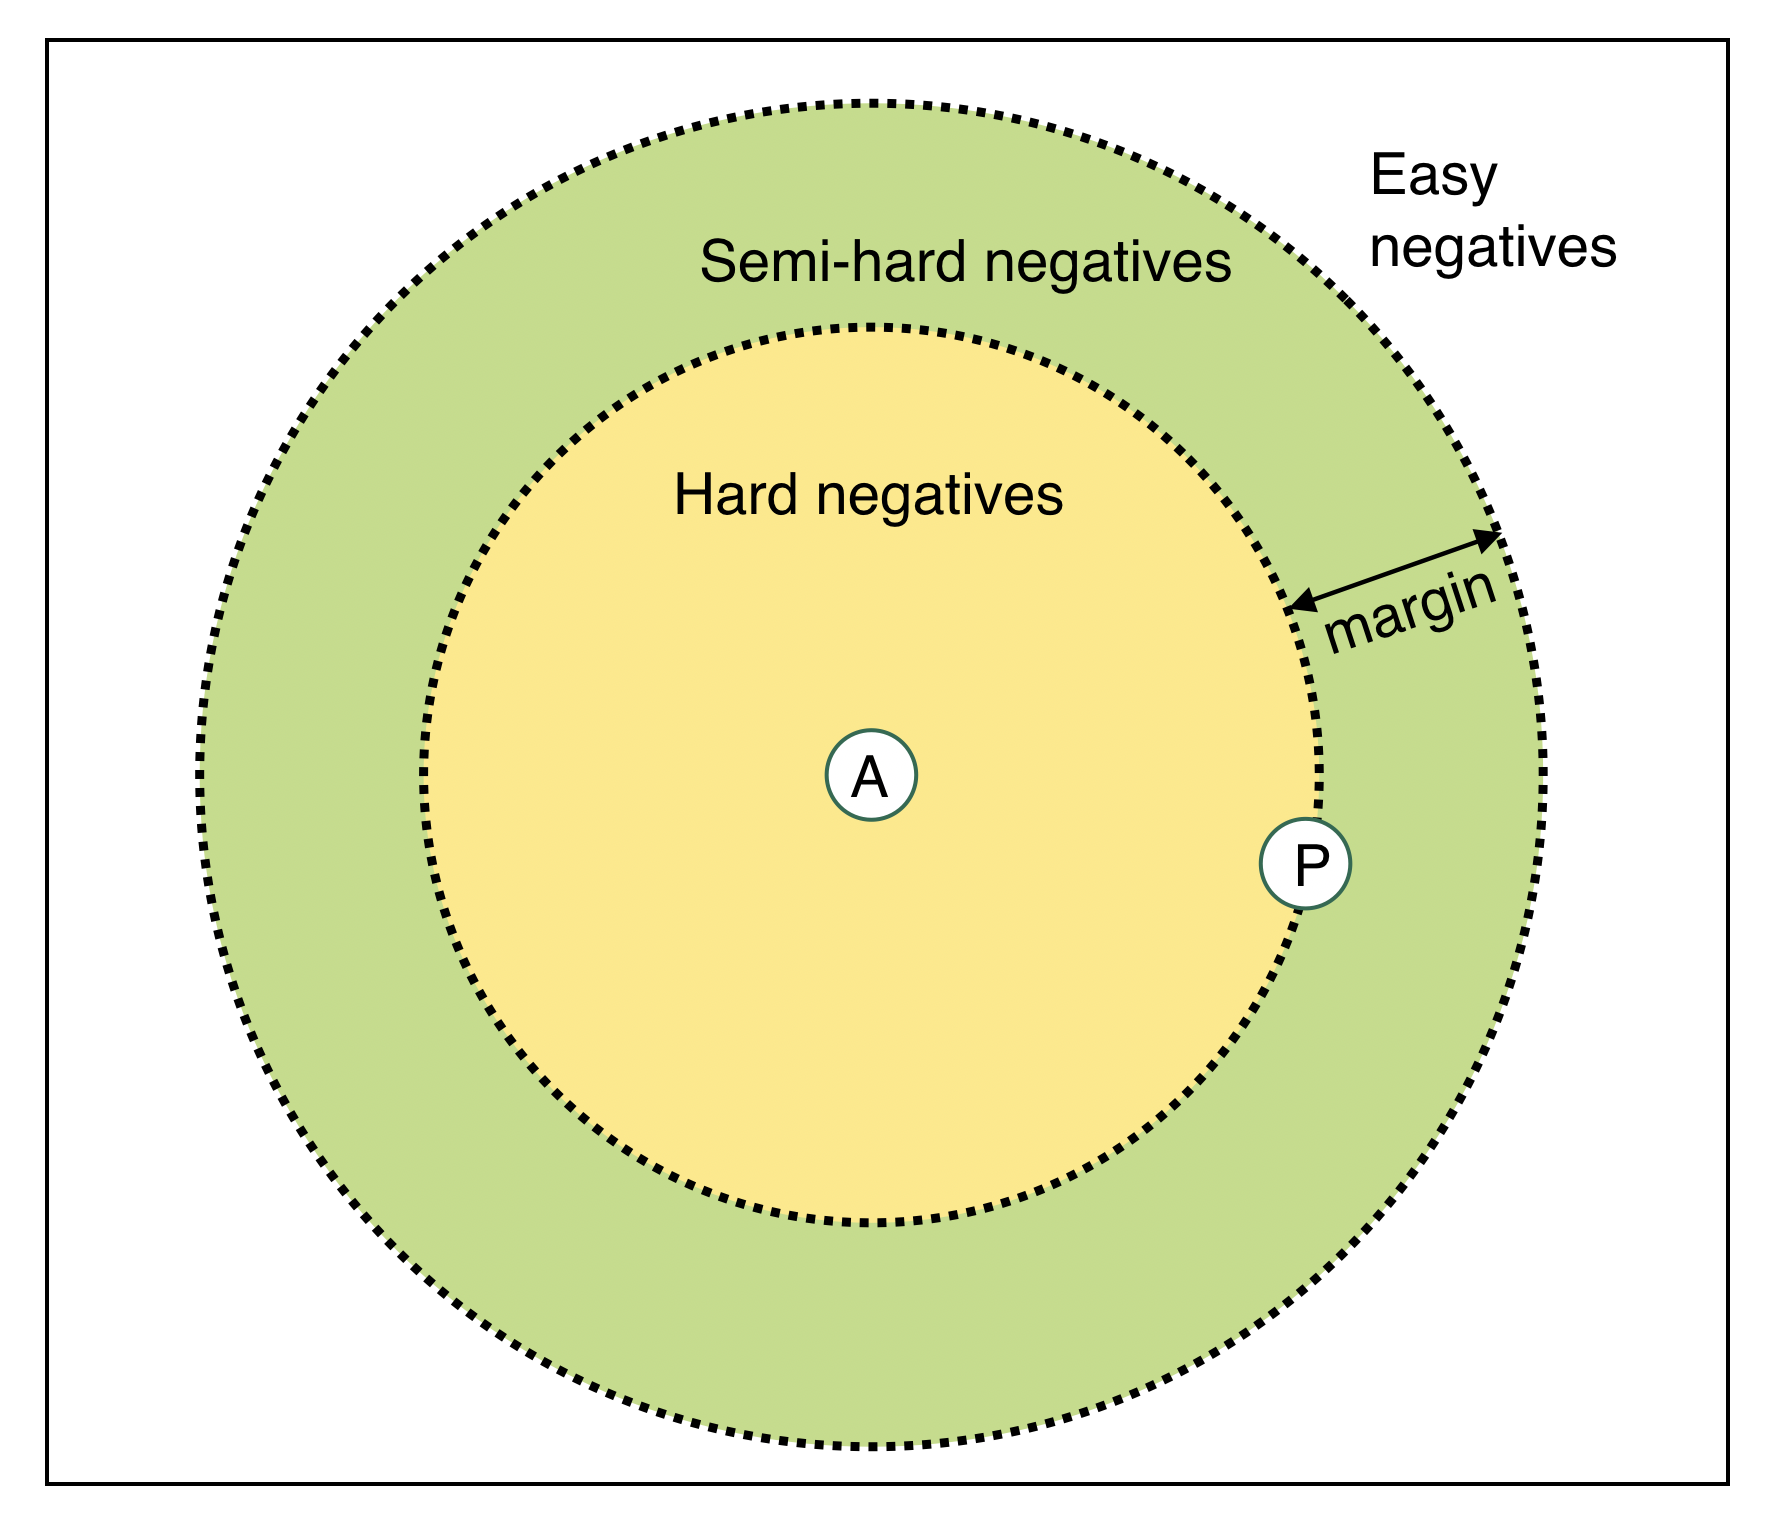
\includegraphics[width=0.6\linewidth]{figs/sitiations.png}
  \caption{Three situations of triplet loss.}
  \label{fig:sitiations}
\end{figure}




